\begin{minipage}{75mm}
The circumcirle of a triangle is the circle intersecting all three vertices. ccRadius returns the radius of the circle going through points A, B and C and ccCenter returns the center of the same circle.
\end{minipage}
\begin{minipage}{15mm}
\vspace{-2mm}
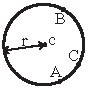
\includegraphics[width=\textwidth]{../code/Geometry/Circle/circumcircle}
\end{minipage}
\begin{minted}{C++}
#include "Point.h"

typedef Point<double> P;
double ccRadius(const P& A, const P& B, const P& C) {
  return (B-A).dist()*(C-B).dist()*(A-C).dist()/
      abs((B-A).cross(C-A))/2;
}
P ccCenter(const P& A, const P& B, const P& C) {
  P b = C-A, c = B-A;
  return A + (b*c.dist2()-c*b.dist2()).perp()/b.cross(c)/2;
}
\end{minted}